
%%%%%%%%%%%%%%%%%%%%%%%%%%%%%%%%%%%%%%%%%%%%%%%%%

% UNIVERSIDADE FEDERAL DO PARANÁ (UFPR)
% SETOR DE CIÊNCIAS SOCIAIS APLICADAS
% PÓS-GRADUAÇÃO EM DESENVOLVIMENTO ECONÔMICO (PPGDE)
% DISCENTE: FELIPE DUPLAT LUZ

%%%%%%%%%%%%%%%%%%%%%%%%%%%%%%%%%%%%%%%%%%%%%%%%%

%%%%%% TRABALHO DE CONCLUSÃO DE CURSO (MONOGRAFIA, DISSERTAÇÃO OU TESE) %%%%%%

%----------------------------------------------------------------
%% Classe abntex2.cls:
%% abntex2.cls, v-1.9.5 laurocesar
%% Copyright 2012-2015 by abnTeX2 group at https://www.abntex.net.br/ 
%%
%----------------------------------------------------------------

% Classe:
\documentclass[
12pt,            % tamanho da fonte.
openright,	     % capítulos começam em pág ímpar (insere página vazia caso preciso).
oneside,         % para impressão em páginas separadas (somente anverso).
%twoside,        % para impressão em anverso (frente) e verso.
a4paper,         % tipo do papel.
chapter=TITLE,   % títulos de capítulos convertidos em letras maiúsculas.
section=TITLE,   % títulos de seções convertidos em letras maiúsculas.
english,         % ENG para hifenização.
spanish,         % ESP para hifenização.
brazil,          % PT-BR para hifenização - o último idioma é o principal do documento
dvipsnames       % cores adicionais.
]{abntex2}

% Estilo do documento:
\usepackage{Arquivos/UFPR}

% Pacotes e formatação:

% ----------------------------------------------------------
% PACOTES BÁSICOS
% ----------------------------------------------------------

\usepackage[T1]{fontenc}		     % seleção de códigos de fonte.
\usepackage[utf8]{inputenc}		     % codificação do documento.
\usepackage{lastpage}		     	 % para a Ficha catalográfica.
\usepackage{indentfirst}     		 % indenta o primeiro parágrafo de cada seção.
\usepackage{color}		         	 % controle das cores.
\usepackage{graphicx}	     		 % inclusão de gráficos.
\usepackage{microtype} 	     		 % para melhorias de justificação.
\usepackage{ifthen}		         	 % para montar condicionais.
\usepackage[brazil]{babel}	     	 % para utilizar termos em portugues.
\usepackage[final]{pdfpages}         % para incluir páginas de arquivos pdf.
\usepackage{lipsum}				     % para gerar dummy text.
\usepackage{csquotes}                % para citações.
%\usepackage[style=long]{glossaries} % para glossário.
%\usepackage{abntex2glossaries}      % para glossário.
\usepackage{cancel} 		         % cancelamento de termos em texto ou equações.
\usepackage{xcolor} 		         % cores estendidas.
\usepackage{smartdiagram}   	     % gera diagramas a partir de listas.
\usepackage{float} 		             % para a figura ficar na posição correta.	    
\usepackage{textcomp} 		         % suporte para fontes da Text Companion. 
\usepackage{longtable}		         % uso de longtable.
\usepackage{amsmath}		         % símbolos matematicos.
\usepackage{lscape}		             % páginas em paisagem.
\usepackage{multicol}		         % mescla de colunas em tabelas.
\usepackage{multirow}		         % mescla de linhas em tabelas.
\usepackage{newfloat} 		         % criação do indice de quadros.
\usepackage{slashbox}                % para tabelas.
\usepackage{makecell}                % para tabelas.

% Para legendas:
%\usepackage{caption}
%[format=plain]
%\renewcommand\caption[1]{
%\captionsetup{font=small}
%,format=hang
%\caption{#1}}
%\captionsetup{width=0.8\textwidth}
\captiondelim{-- }
\captiontitlefont{\small}
\captionnamefont{\small}



% ----------------------------------------------------------
% FORMATAÇÃO
% ----------------------------------------------------------

% BibLaTeX:
\usepackage[
style=abnt,
backref=true,
backend=biber,
citecounter=true,
backrefstyle=three, 
url=true,
maxbibnames=99,
mincitenames=1,
maxcitenames=3,
backref=false,
hyperref=true,
giveninits=true,
uniquename=false,
uniquelist=false]{biblatex}

% Espaçamento entre os itens nas referências:
%\setlength\bibitemsep{\baselineskip}

% Texto padrão para as referências:
\DefineBibliographyStrings{brazil}{%
	 backrefpage  = {Citado \arabic{citecounter} vez na página},
	 backrefpages = {Citado \arabic{citecounter} vezes nas páginas},
	 urlfrom      = {Dispon\'ivel em},
}

% Indentação de referências:
\defbibheading{bay}[\bibname]{
\chapter*{#1}
\markboth{#1}{#1}%
\addcontentsline{toc}{chapter}
%{\protect\numberline{}\bibname}
{\bibname}}

% Formatando o avanço dos títulos no sumário:
\makeatletter
	\pretocmd{\chapter}{\addtocontents{toc}{\protect\addvspace{-12\p@}}}{}{}
	\pretocmd{\section}{\addtocontents{toc}{\protect\addvspace{-3\p@}}}{}{}
\makeatother


% Inserir maiúsculo na seção:
% (https://groups.google.com/g/abntex2/c/ZYwE4t9uTFM)
\makeatletter
\let\oldcontentsline\contentsline
\def\contentsline#1#2{%
	\expandafter\ifx\csname l@#1\endcsname\l@section
	\expandafter\@firstoftwo
	\else
	\expandafter\@secondoftwo
	\fi
	{%
		\oldcontentsline{#1}{\MakeTextUppercase{#2}}%
	}{%
		\oldcontentsline{#1}{\MakeTextUppercase{#2}}%
	}%
}
\makeatother

% Retirar os símbolos <> da URL:
\DeclareFieldFormat{illustrated}{\addspace #1\isdot}
%\DeclareFieldFormat{url}{\bibstring{urlform}\addcolon\addspace<\url{#1}>}
%\DeclareFieldFormat{url}{\bibstring{urlfrom}\addcolon\addspace<\url{#1}>}
\DeclareFieldFormat{url}{\bibstring{urlfrom}\addcolon \space\addspace{#1}}

% Ajustar o espaço para a formatação da data:
\DeclareFieldFormat{urldate}{\bibstring{urlseen}\addcolon\addspace #1}%
\DeclareFieldFormat*{note}{\addspace #1}%

% Ajustar o tamanho da fonte do número da primeira página do capítulo (na parte textual):
\makepagestyle{chapfirst}
\makeoddhead{chapfirst}{}{}{\footnotesize{\thepage}}

% Novo estilo de cabeçalhos e rodapés:
\makepagestyle{simplestextual}

% Cabeçalho para página par:
\makeevenhead{simplestextual}
  {}{}{\footnotesize \thepage}

% Cabeçalho para página ímpar:
\makeoddhead{simplestextual} %%pagina ímpar ou com oneside
  {}{}{\footnotesize \thepage}

% Linha no rodapé:  
%\makeheadrule{simplestextual}{\textwidth}{\normalrulethickness}

% Rodapé:
\makeevenfoot{simplestextual}
  {}{}{} %%pagina par

% Página ímpar ou com oneside:      
\makeoddfoot{simplestextual}
  {}{}{}

% Formatação dos capítulos póstextuais numerados:
%\newcommand{\refap}[1]{\hyperref[#1]{Apêndice~\ref{#1}}} 	% Referência apÊndices

% uso do tikz e pgfplots:
%\usetikzlibrary{external}
\usetikzlibrary{arrows,calc,patterns,angles,quotes}
\usepackage{pgfplots}
\pgfplotsset{compat=1.15}

% Define o comando para citação de fontes em elementos gráficos:
\newcommand{\citefig}[2]{~\Citeauthor*{#1}\citeyear{#1}}

% Define os operadores matemáticos em português:
\DeclareMathOperator{\tr}{tr}
\DeclareMathOperator{\sen}{sen}
\DeclareMathOperator{\senh}{senh}
%\DeclareMathOperator{\tag}{tag}
\DeclareMathOperator{\tg}{tg}
\DeclareMathOperator{\tagh}{tagh}
\DeclareMathOperator{\tgh}{tgh}
\DeclareMathOperator{\cossec}{cossec}
%\DeclareMathOperator{\sen}{sen}

% Listagem de codigos LaTeX na documentação:
\usepackage{listings}

% Citação de documentos não publicados e informais e colocar nas notas de rodapé:
\newcommand{\citenp}[1]{
\cite{#1}\footnote{\fullcite{#1}}}

\newcommand{\textcitenp}[1]{
	\textcite{#1}\footnote{\fullcite{#1}}}




% Informações do documento:

% ----------------------------------------------------------
% DADOS
% ----------------------------------------------------------

% Tipo de TCC (Monografia, Dissertação, Tese ou Relatório Técnico):
\tipotrabalho{Dissertação}

% Informações do TCC:
\titulo{título do trabalho} % título.
\autor{autor do trabalho}                % autor.
\local{Cidade}                           % cidade.
\data{Ano}                               % ano.
\orientador{Orientador(a)}               % orientador  - se homem.
%\orientadora{}                          % orientadora - se mulher.
%\coorientador{}                         % co-orientador  - se homem
%\coorientadora{Kênia Barreiro de Souza} % co-orientadora - se mulher
%\scoorientador{}                        % segundo co-orientador  - se mulher
%\scoorientadora{}                       % segunda co-orientadora - se mulher

% Adicionar referências:
\addbibresource{Arquivos/Referências.bib}

% Cabeçalho da capa:
\instituicao{Universidade Federal do Paraná}
\def \ImprimirSetor{Setor de Ciências Sociais Aplicadas}
\def \ImprimirProgramaPos{Programa de Pós-Graduação em Desenvolvimento Econômico}
\def \ImprimirCurso{}
\preambulo{Dissertação/Tese de mestrado/doutorado apresentada ao Programa de Pós-Graduação em Desenvolvimento Econômico do Setor de Ciências Sociais Aplicadas da Universidade Federal do Paraná como requisito parcial para obtenção do título de mestre/doutor em Desenvolvimento Econômico}

% Informações complementares:
\newcommand{\imprimirCurso}{}
\newcommand{\imprimirDataDefesa}{Data da defesa}
\newcommand{\imprimircdu}{02:141:005.7}

% Comandos de dados - Data da apresentação
\providecommand{\imprimirdataapresentacaoRotulo}{}
\providecommand{\imprimirdataapresentacao}{}
\newcommand{\dataapresentacao}[2][\dataapresentacaoname]{\renewcommand{\dataapresentacao}{#2}}

% Comandos de dados - Nome do Curso
\providecommand{\imprimirnomedocursoRotulo}{}
\providecommand{\imprimirnomedocurso}{}
\newcommand{\nomedocurso}[2][\nomedocursoname]
  {\renewcommand{\imprimirnomedocursoRotulo}{#1}
\renewcommand{\imprimirnomedocurso}{#2}}






% ----------------------------------------------------------
% DADOS INICIAIS
% ----------------------------------------------------------

\begin{document}

% Uppercase dos títulos:
\renewcommand{\tablename}{TABELA}
\renewcommand{\figurename}{FIGURA}
\renewcommand{\figureautorefname}{FIGURA}
\renewcommand{\tableautorefname}{TABELA}
\newcommand{\equationname}{EQUA\c{C}\~AO~}
\renewcommand{\equationautorefname}{EQUA\c{C}\~AO~}
\renewcommand{\bibname}{{REFER\^ENCIAS}}
\renewcommand{\apendicesname}{Ap\^endices}
\renewcommand{\anexosname}{Anexos}

% Fonte do número da primeira página do capítulo:
\aliaspagestyle{chapter}{chapfirst}



% ----------------------------------------------------------
% ELEMENTOS PRÉ-TEXTUAIS
% ----------------------------------------------------------
\pretextual


%---------------------------------------------------------------------
% CAPA
%---------------------------------------------------------------------

\renewcommand{\imprimircapa}{%
	\begin{capa}%
		\center
		\begin{tikzpicture}[remember picture,overlay] 
			\node[anchor=south west, yshift= 25mm, xshift=-1.5mm] at 
			(current page.south west) 
			{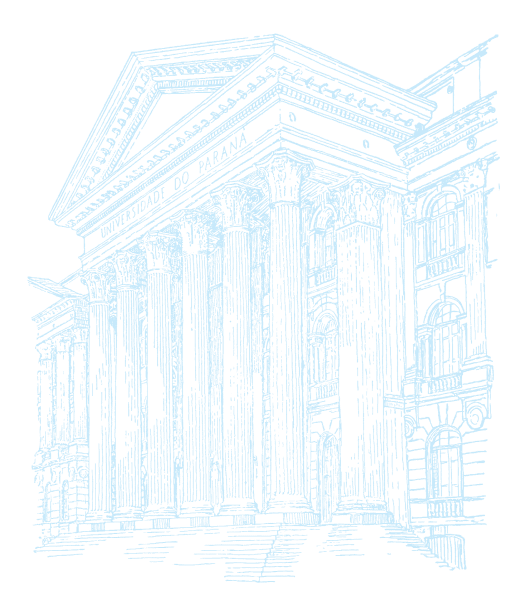
\includegraphics[width = \paperwidth]{Imagens/capa_UFPR}};
		\end{tikzpicture}
		\center
		%    \ABNTEXchapterfont 
		\MakeUppercase\imprimirinstituicao \vspace{-2mm}
		
		\ifthenelse{\equal \ImprimirSetor{}}{}{
			%    \ABNTEXchapterfont 
			\MakeUppercase\ImprimirSetor}
		\vspace{-2mm}
		
		\ifthenelse{\equal \ImprimirProgramaPos{}}{}{
			%    \ABNTEXchapterfont 
			\MakeUppercase\ImprimirProgramaPos}
		
		\ifthenelse{\equal \ImprimirCurso{}}{}{
			%    \ABNTEXchapterfont 
			\MakeUppercase\ImprimirCurso}
		
		\vspace{40mm}
		
		%    \ABNTEXchapterfont 
		\MakeUppercase\imprimirautor
		
		\vspace{40mm}
		%    \ABNTEXchapterfont
		\MakeUppercase\imprimirtitulo
		\vfill
		
		%\large
		\MakeUppercase\imprimirlocal
		
		%\large
		\imprimirdata
		
		\vspace*{10mm}
	\end{capa}
}

\imprimircapa


                             % Capa.

%---------------------------------------------------------------------
% FOLHA DE ROSTO
%---------------------------------------------------------------------

\makeatletter
\renewcommand{\folhaderostocontent}{
	\begin{center}
		
		%\vspace*{1cm}
		{
			%\ABNTEXchapterfont
			%\large
			\MakeUppercase\imprimirautor}
		
		\vspace*{\fill}%\vspace*{\fill}
		\begin{center}
			%      \ABNTEXchapterfont
			%\bfseries
			%\Large
			\MakeUppercase\imprimirtitulo
		\end{center}
		\vspace*{\fill}
		
		\abntex@ifnotempty{\imprimirpreambulo}{%
			\hspace{.45\textwidth}
			\begin{minipage}{.5\textwidth}
				\SingleSpacing\small
				\imprimirpreambulo.\vspace*{2mm}
				
				\abntex@ifnotempty{\imprimirorientador}
				{\imprimirorientadorRotulo~\imprimirorientador}
				\ifthenelse{\equal{\imprimirorientador}{}}
				{\imprimirorientadoraRotulo~\imprimirorientadora}
				{}
				\abntex@ifnotempty{\imprimircoorientador}
				{\par\imprimircoorientadorRotulo~\imprimircoorientador}%
				{\abntex@ifnotempty{\imprimircoorientadora}
					{\par\imprimircoorientadoraRotulo~\imprimircoorientadora}%
				}
				\ifthenelse{\equal{\imprimirscoorientadora}{} \AND \equal{\imprimirscoorientador}{}}{}
				{
					\ifthenelse{\equal{\imprimirscoorientador}{}}{}
					{\par\imprimirscoorientadorRotulo~\imprimirscoorientador}
					\ifthenelse{\equal{\imprimirscoorientadora}{}}{}
					{\par\imprimirscoorientadoraRotulo~\imprimirscoorientadora}
				}%
				%
			\end{minipage}%
			\vspace*{\fill}
		}%
		
		\vspace*{\fill}
		
		
		{  \MakeUppercase\imprimirlocal}
		\par
		{    \imprimirdata}
		\vspace*{1cm}
		
	\end{center}
}
\makeatother

\imprimirfolhaderosto*


                   % Folha de rosto.

%---------------------------------------------------------------------
% FICHA CATALOGRÁFICA
%---------------------------------------------------------------------

% São duas opções possíveis: usar um PDF pronto ou usar o comando abaixo. Se quiser usar o PDF, basta inserir um arquivo .pdf na pasta "Pré" chamado "Ficha catalográfica". Caso queira usar o comando, basta editá-lo abaixo de acordo com suas necessidades e depois remover o .pdf da pasta "Pré".

\newcommand{\PalavraschaveTexto}{Palavra 01. Palavra 02. Palavra 03.}

\newcommand{\insereFichaCatalografica}{ 
		\IfFileExists{Pré/Ficha_catalográfica.pdf}
		{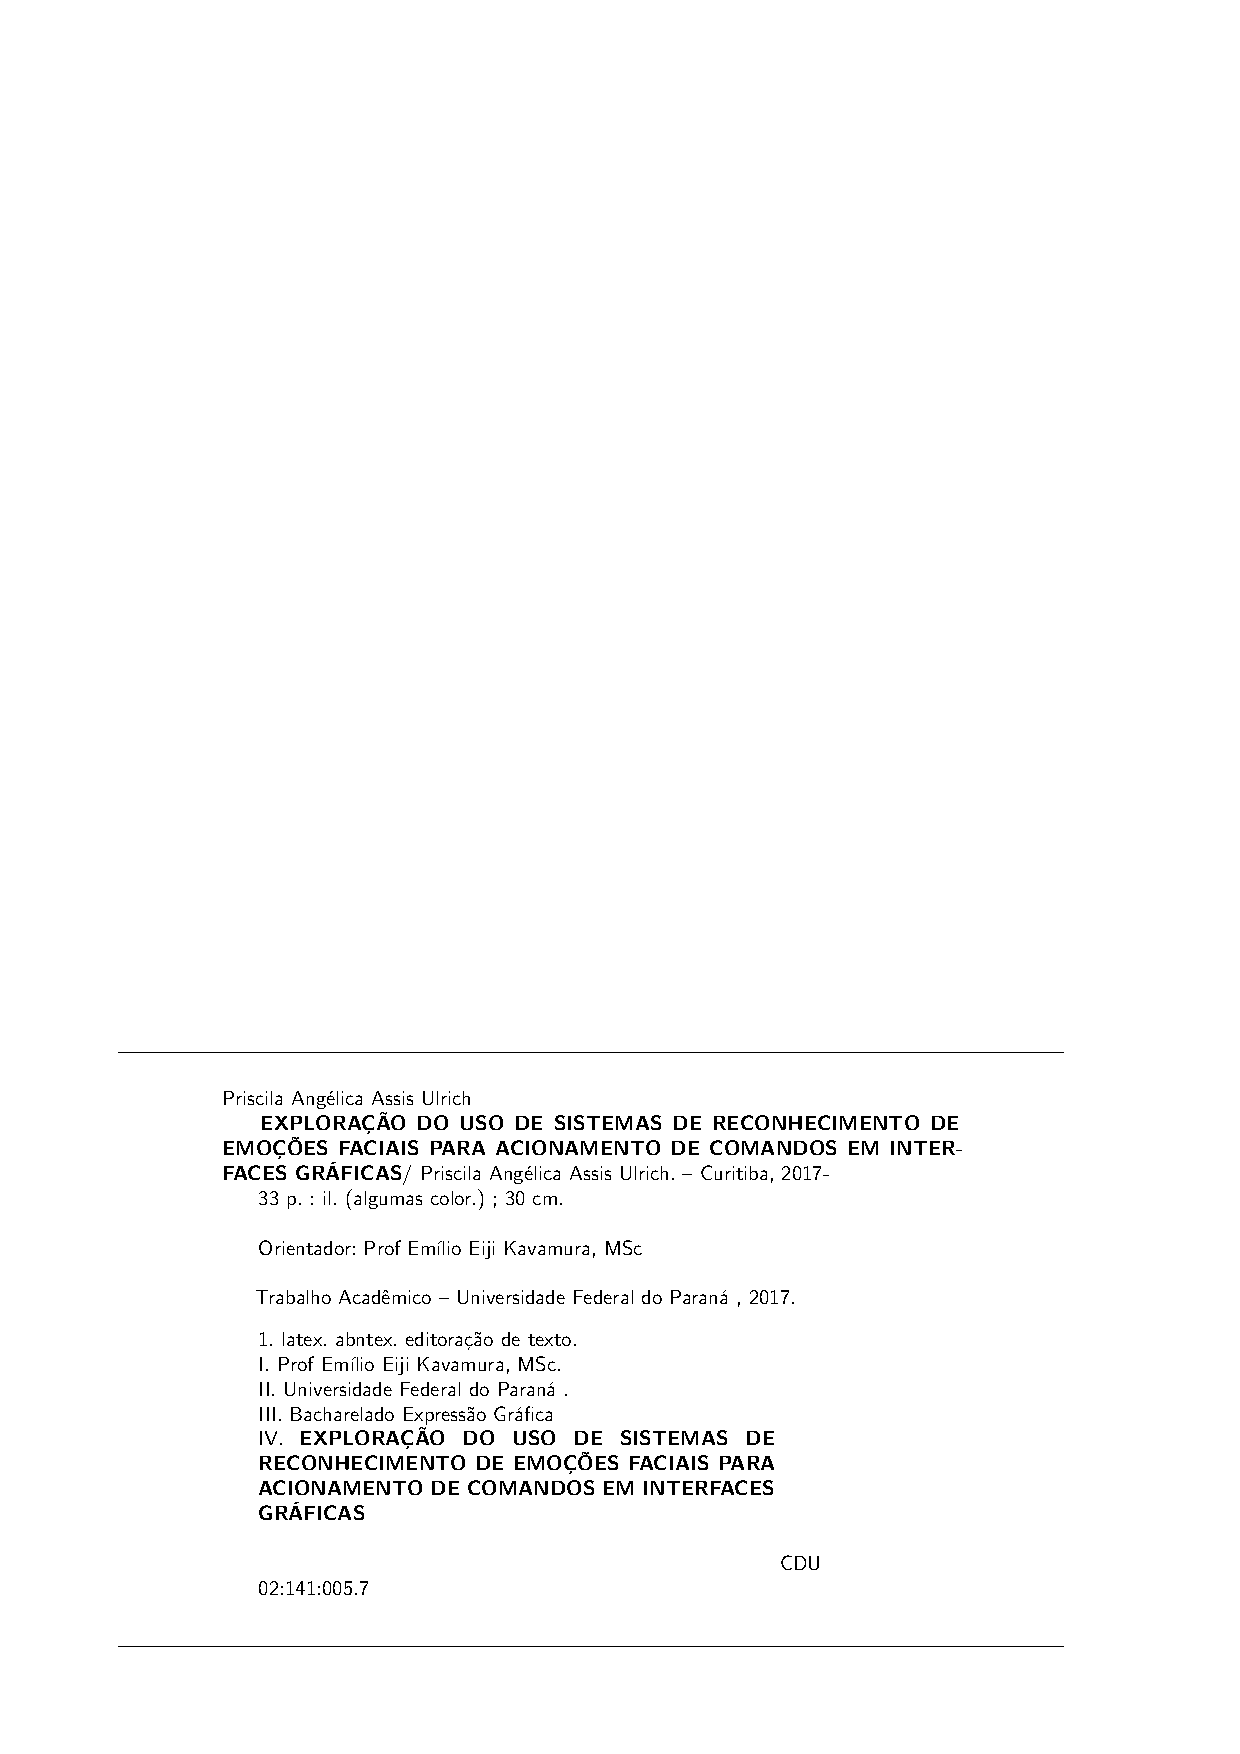
\includepdf[pages=-]{Pré/Ficha_catalográfica.pdf}}
		{
			\begin{fichacatalografica}%\color{blue}
			\vspace*{\fill}					% Posição vertical
			\hrule							% Linha horizontal
			\begin{center}					% Minipage Centralizado
				\begin{minipage}[c]{12.5cm}		% Largura
					
					\imprimirautor
					
					\hspace{0.5cm} \imprimirtitulo  / \imprimirautor. --
					\imprimirlocal, \imprimirdata.
					
					\hspace{0.5cm} \pageref{LastPage} p. : il. color \\
					
					\hspace{0.5cm} \imprimirtipotrabalho (mestrado) - \imprimirinstituicao. \ImprimirProgramaPos, do \ImprimirSetor. \\ 
					
					\hspace{0.5cm} Orientador: \imprimirorientador \\
					
					\hspace{0.5cm} Coorientadora: \imprimircoorientadora \\
					
					\hspace{0.5cm} Defesa: \imprimirlocal, \imprimirdata. \\
					
					\begin{minipage}{.96\textwidth}
						\hspace{0.5cm} 1. \PalavraschaveTexto. I. \imprimirinstituicao. \ImprimirSetor. \ImprimirProgramaPos. II. \imprimirorientador. III. \imprimircoorientadora. IV. \imprimirtitulo\\ 
						
						\hspace{92mm} CDU \imprimircdu \\
					\end{minipage}
				\end{minipage}
			\end{center}
			\hrule
		\end{fichacatalografica}
	}
}

\insereFichaCatalografica
\cleardoublepage


             % Ficha catalográfica.

%---------------------------------------------------------------------
% ERRATA
%---------------------------------------------------------------------

Elemento opcional:
	\vspace{\onelineskip}
	
	FERRIGNO, C. R. A. \textbf{Tratamento de neoplasias ósseas apendiculares com
		reimplantação de enxerto ósseo autólogo autoclavado associado ao plasma
		rico em plaquetas}: estudo crítico na cirurgia de preservação de membro em
	cães. 2011. 128 f. Tese (Livre-Docência) - Faculdade de Medicina Veterinária e
	Zootecnia, Universidade de São Paulo, São Paulo, 2011.
	
	\begin{table}[htb]
		\center
		\footnotesize
		\begin{tabular}{|p{1.4cm}|p{1cm}|p{3cm}|p{3cm}|}
			\hline
			\textbf{Folha} & \textbf{Linha}  & \textbf{Onde se lê}  & \textbf{Leia-se}  \\
			\hline
			1 & 10 & auto-conclavo & autoconclavo\\
			\hline
		\end{tabular}
\end{table}


                          % Errata.

%---------------------------------------------------------------------
% TERMO DE APROVAÇÃO
%---------------------------------------------------------------------

% São duas opções possíveis: usar um PDF pronto ou usar o comando abaixo. Se quiser usar o PDF, basta inserir um arquivo .pdf na pasta "Pré" chamado "Termo de aprovação". Caso queira usar o comando, basta editá-lo abaixo de acordo com suas necessidades e depois remover o .pdf da pasta "Pré".

\newcommand{\insereAprovacao}{
	\IfFileExists{Pré/Termo de aprovação.pdf}
	{\includepdf[pages=-]{Pré/Termo de aprovação.pdf}}
	{
		\begin{folhadeaprovacao}%\color{blue}
			
			\begin{center}
				{\ABNTEXchapterfont
					{\large\bfseries\MakeUppercase\folhadeaprovacaoname}\par\phantom{}\par
					%\large
					\MakeUppercase\imprimirautor}
				
				\vspace*{\fill}\vspace*{\fill}
				\begin{center}
					\ABNTEXchapterfont
					%\bfseries\Large
					\MakeUppercase\imprimirtitulo
				\end{center}
				\vspace*{\fill}
				\begin{minipage}{\textwidth}
					\hspace{.45\textwidth}
					\begin{minipage}{.5\textwidth}
						\imprimirpreambulo pela seguinte banca examinadora:
					\end{minipage}%
				\end{minipage}
				
				
				\vspace*{\fill}
			\end{center}
			\assinatura{{
					\ifthenelse{\equal{\imprimirorientador}{}}
					{\imprimirorientadora \\ Orientadora}
					{\imprimirorientador \\ Orientador}}
			}
			\assinatura{
				{Kênia Barreiro de Souza} \\ Co-orientadora}
			\assinatura{%\textbf
				{Professor(a)} \\ Universidade XXX}
			\assinatura{%\textbf
				{Professor(a)} \\ Universidade XXX}
			%\assinatura{%\textbf{Professor} \\ Convidado 4}
			
			\begin{center}
				\vspace*{0.5cm}
				%{\large\imprimirlocal}
				%\par
				%{\large\imprimirdata}
				\imprimirlocal, \imprimirDataDefesa.
				\vspace*{1cm}
			\end{center}
			
		\end{folhadeaprovacao}
	}
}

\insereAprovacao


              % Termo de aprovação.

%---------------------------------------------------------------------
% DEDICATÓRIA
%---------------------------------------------------------------------

\begin{dedicatoria}
	\vspace*{\fill}
	\centering
	\noindent
	
	\textit{Eu dedico...}
	
	\vspace*{\fill}
\end{dedicatoria}


                     % Dedicatória.

%---------------------------------------------------------------------
% AGRADECIMENTOS
%---------------------------------------------------------------------

\begin{agradecimentos}
	Texto.
\end{agradecimentos}


                  % Agradecimentos.

%---------------------------------------------------------------------
% EPÍGRAFE
%---------------------------------------------------------------------

\begin{epigrafe}
	\vspace*{\fill}
	\begin{flushright}
		\textit{``as  elites são patrimonialistas e conservadoras, a classe média \\ é meritocrática e o povo? o povo não é nada!''}
	\end{flushright}
\end{epigrafe}


                        % Epígrafe.

\documentclass{article}

% Pacotes utilizados:
\usepackage{titlesec}              % permitir versalete na seção.
\usepackage[T1]{fontenc}           % codificar fonte.
\usepackage[bindingoffset=0.2in,
left=1in,
right=1in,
top=1in,
bottom=1.5in,
footskip=.25in]{geometry}          % configurar margens.
\usepackage{amsmath}               % pacote matemático.
\usepackage{amssymb}               % pacote matemático.
\usepackage{txfonts}               % fonte Times New Roman.
\usepackage{graphicx}              % inserir imagens.
\usepackage[brazil]{babel}         % deixar em pt-br.
\usepackage[style = abnt,          % manter formato ABNT.
            giveninits,            % manter primeiros nomes abreviados.
            scbib                  % manter em versalete.
]{biblatex}                        % adicionar referências.
\usepackage{makecell}              % quebrar linha da tabela.

% Referências:
\addbibresource{Referências.bib}

% Seções do texto:
\titleformat{\section}
{\scshape\bfseries\Large}
{}
{0em}
{}	
[]

% Cabeçalho:
\title{\textbf{\textsc{Título}} \\ \Large \textsc{Subtítulo}}
\author{\textsc{Felipe Duplat Luz}}
\date{\textsc{\today}}

% Configurações:
\setlength\parindent{0pt}
\setlength{\textwidth}{18cm} 
\setlength{\oddsidemargin}{-0.7cm}



%---

% Início do documento:
\begin{document}
	\maketitle
	
\section*{Resumo}
\setlength\parskip{0.3cm}

Texto. \cite{jones71,samuelson71}



%Referências:
\pagebreak
\printbibliography[title={Referências:}]



\end{document}


                           % Resumo.

%---------------------------------------------------------------------
% ABSTRACT
%---------------------------------------------------------------------

% ENG:
\begin{resumo}[Abstract]
	\begin{otherlanguage*}{english}
		\SingleSpacing
		
		Text.
		
		\noindent 
		\textbf{Keywords}: . \\
		\textbf{JEL Classification}: .
	\end{otherlanguage*}
\end{resumo}


                         % Abstract.

%---------------------------------------------------------------------
% LISTAS
%---------------------------------------------------------------------

% Lista de figuras:
\pdfbookmark[0]{\listfigurename}{lof}
\listoffigures*
\cleardoublepage



% Lista de quadros:
\pdfbookmark[0]{\listtablename}{lot}
\listofquadros*
\cleardoublepage



% Lista de tabelas:
\pdfbookmark[0]{\listtablename}{lot}
\listoftables*
\cleardoublepage



% Lista de abreviaturas e símbolos:
\begin{siglas}
	
	\item[ECV] Esporte Clube Vitória.
	
	\item[]     
	
\end{siglas}


% Símbolos:
\begin{simbolos}
	\item[$\alpha$] Letra grega Alfa em minúsculo.
	\item[$\beta$]  Letra grega Beta em minúsculo.
	\item[$\gamma$] Letra grega gama em minúsculo.
\end{simbolos}



% Sumário:
%\pdfbookmark[0]{\contentsname}{toc}
\phantompart \tableofcontents*
%\cleardoublepage


                           % Listas de figuras, quadros, tabelas e sumário.



% ----------------------------------------------------------
% ELEMENTOS TEXTUAIS
% ----------------------------------------------------------
\textual


% ----------------------------------------------------------
% CAPÍTULO 01 - INTRODUÇÃO
% ----------------------------------------------------------

\chapter{Introdução} \label{cha:introdução}

\section{Teste} \label{sec:teste}

Texto \cite{anderson20, campostimini22, do09}.




% ----------------------------------------------------------
% CAPÍTULO 02 - Revisão de literatura
% ----------------------------------------------------------

\chapter{Revisão de literatura}

Texto.

% ----------------------------------------------------------
% CAPÍTULO 03 - METODOLOGIA E DADOS
% ----------------------------------------------------------

\chapter{Metodologia e dados} \label{cha:metodologia}

Texto.




% ----------------------------------------------------------
% CAPÍTULO 04 - RESULTADOS
% ----------------------------------------------------------

\chapter{Resultados}

Texto.


	


% ----------------------------------------------------------
% CAPÍTULO 05 - CONSIDERAÇÕES FINAIS
% ----------------------------------------------------------

\chapter{Considerações finais}

Texto.






% ----------------------------------------------------------
% ELEMENTOS PÓS-TEXTUAIS
% ----------------------------------------------------------
\postextual

% Referências:
\begingroup
\printbibliography[title = Referências, heading = bibintoc, notkeyword = {consulta}, notkeyword={npub-informal}]
\endgroup

% Capítulos pós-textuais:
%\addtocontents{toc}{\vspace{4pt}}

% Apêndice:

%---------------------------------------------------------------------
% APÊNDICE
%---------------------------------------------------------------------


\chapter{Apêndice 01}
\label{ap:ap01}

\lipsum[1-2]





% Anexo:

%---------------------------------------------------------------------
% ANEXO
%---------------------------------------------------------------------

\begin{anexosenv}
	\renewcommand{\thechapter}{\arabic{chapter}}
	\partanexos
	\chapter{Título} \label{an:an01}
	
	Texto.
	
\end{anexosenv}




\end{document}


